\subsection{UC2 - Inizializzazione Metadati}
\label{sub:uc2}

\begin{figure}[h]
    \centering
    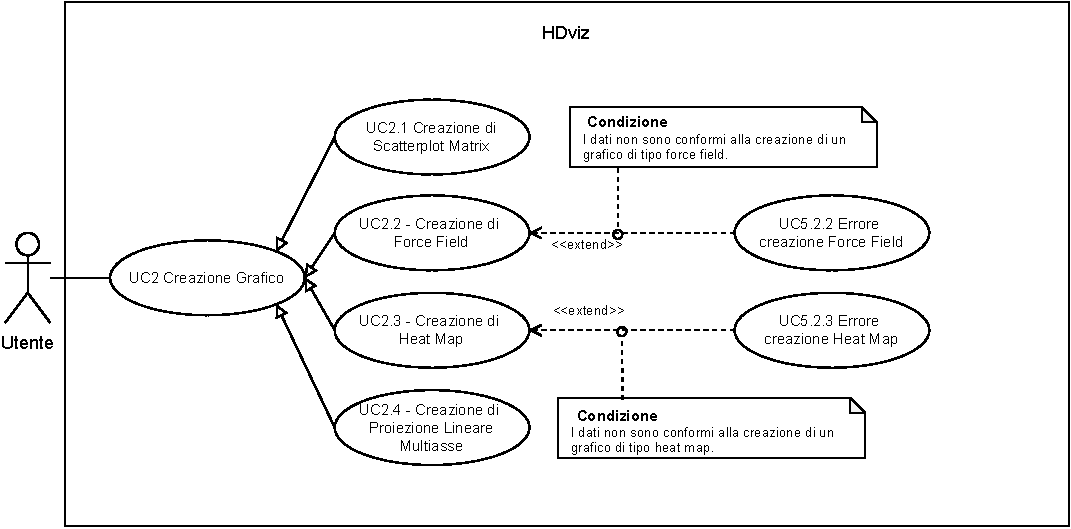
\includegraphics[width=0.5\textwidth]{componenti/casi-duso/diagrammi/UC2.pdf}
    \caption{Diagramma rappresentante UC2}
    \label{fig:UC2}
\end{figure}

\begin{itemize}
	\item \textbf{Descrizione}: L'utente assegna ad ogni riga del dataset precedentemente caricato
								un metatag che ne descrivi la tipologia di dato;
	
	\item \textbf{Attore primario}: Utente;
	\item \textbf{Precondizione}: 	I dati sono stati correttamente importati e non hanno ancora alcun
									metatag assegnato
	\item \textbf{Postcondizione}:  Ai dati sono stati assegnati dei metatag assegnati dall'utente 

	\item \textbf{Scenario principale}:
		\begin{enumerate}
			\item L'utente seleziona l'opzione di aggiunta dei metatag;
			\item Per ogni header del dataset può selezionare il tipo di metadati più adatto mediante menu a tendina;
		\end{enumerate}
\end{itemize}

